\documentclass{article}

\usepackage[submission]{colm2026_conference}
\usepackage{microtype}
\usepackage{hyperref}
\usepackage{url}
\usepackage{booktabs}
\usepackage{graphicx}
\usepackage{amsmath}
\usepackage{lineno}

\definecolor{darkblue}{rgb}{0, 0, 0.5}
\hypersetup{colorlinks=true, citecolor=darkblue, linkcolor=darkblue, urlcolor=darkblue}
\Urlmuskip=0mu plus 2mu\relax

\title{Fixed-Byte Source-Private Candidate Packets for Bounded Model Collaboration}

\author{Anonymous authors\\Paper under double-blind review}

\newcommand{\method}{LatentWire}
\newcommand{\arc}{ARC-Challenge}
\newcommand{\obqa}{OpenBookQA}

\begin{document}

\ifcolmsubmission
\linenumbers
\fi

\maketitle

\begin{abstract}
Multi-model language systems usually communicate by emitting text or by sharing internal state such as KV caches. Text is portable but slow and lossy; cache sharing is information-rich but exposes thousands of bytes of model state per token and requires architecture-specific machinery. We study a narrower question: can a frozen source model send a fixed-byte, source-private candidate packet that improves a frozen receiver on public multiple-choice reasoning tasks, without sending source text, hidden states, KV cache, source logits, or gold labels? We present \method, a public-coordinate packet protocol in which source and receiver agree on an anchor/spectral basis over candidate answers, the source emits a tiny signed packet, and the receiver decodes the packet against its own public side information. On \arc{} test, an 8-byte packet reaches 0.344 accuracy across 10 seeds, above target-only 0.265 and same-byte structured text 0.300, with destructive coordinate controls failing in all 10 seeds; the source-choice accuracy is 0.346, so the positive should be read as compact source-candidate transfer rather than evidence synthesis beyond the source. On \obqa{} test, a 3-byte packet reaches 0.378 across 5 seeds, above target-only 0.276 and same-byte text 0.350, matching the source-choice accuracy. We also report strict negative evidence: a Phi-3 cross-family source fails the same gate, and learned cache/score connectors built from available cached artifacts do not repair it. The contribution is therefore not a universal latent language claim and does not beat explicit source-index communication. It is a reproducible fixed-byte source-private transfer result, a falsification protocol for cross-family claims, and a systems accounting boundary showing that task packets are 69.8x smaller than even a one-token 1-bit-per-KV-element accounting floor.
\end{abstract}

\section{Introduction}

Future language-model systems will often use more than one model: a cheap model may screen candidates, a specialist may inspect hard cases, and a stronger receiver may combine evidence. The simplest interface is text. Recent cache-level systems instead communicate through model internals, such as fused or selectively shared KV caches~\citep{Fu2025C2C,Shi2025KVComm}. These approaches are powerful, but they couple communication to large hidden-state objects and serving substrates.

This paper asks whether a much smaller interface can carry useful source-side candidate evidence. In our setting, both models see the same public question and answer choices. The source performs private computation over those choices. The only communicated object is a short byte packet; the receiver never sees source text, source logits, source hidden vectors, KV cache, or the answer key. This is a side-information problem in the spirit of distributed source coding~\citep{Slepian1973Noiseless,Wyner1976RateDistortion}: the receiver already has the public prompt and its own computation, so the packet should carry only the source evidence that is useful at the decoder.

Our strongest current result is deliberately scoped. On \arc{} and \obqa{}~\citep{Clark2018ARC,Mihaylov2018OpenBookQA}, same-family Qwen2.5 packet transfer~\citep{Yang2025Qwen25} improves over target-only and same-byte text controls. However, a strict Phi-3 source-family replacement~\citep{Abdin2024Phi3} fails, and additional connector repairs fail on the available cached artifacts. This boundary matters: the paper is not claiming solved cross-family latent communication.

The contributions are:
\begin{itemize}
\item A fixed-byte, source-private packet protocol for multiple-choice candidate transfer with no source text, hidden vector, KV cache, source-logit, or gold-label exposure.
\item A public-coordinate anchor/spectral implementation that is positive on \arc{} and \obqa{} under seed repeats, paired uncertainty, same-byte text controls, and destructive coordinate mismatch controls.
\item A source-choice and falsification audit showing that the current positive is mostly source-choice preserving and same-family/source-cache specific: Phi-3 cross-family transfer and cached learned repair connectors fail.
\item A systems accounting artifact comparing packet bytes and exposure classes against KV/cache communication and KV quantization floors, while explicitly separating byte accounting from native serving-speed claims.
\end{itemize}

\begin{figure}[t]
  \centering
  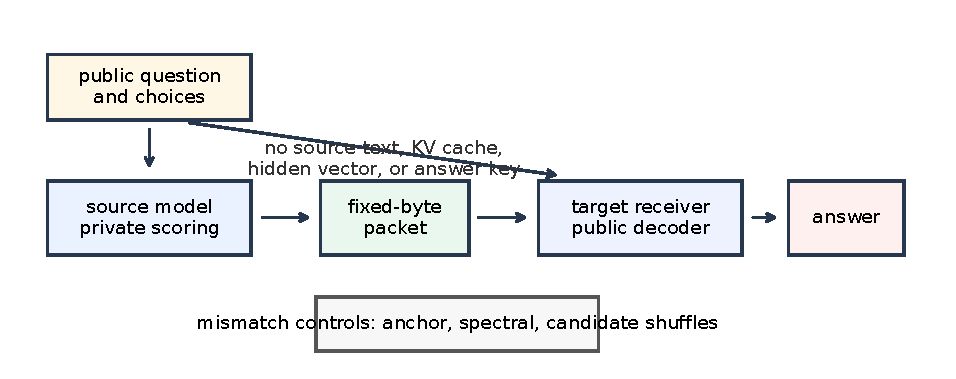
\includegraphics[width=0.96\linewidth]{figures/protocol_diagram.pdf}
  \caption{\method{} protocol. Both sides receive the public task. The source privately scores candidates and emits only a fixed-byte packet. The receiver decodes the packet with a public basis and its own side information. Destructive controls scramble the shared coordinate system or candidate relation.}
  \label{fig:protocol}
\end{figure}

\section{Source-private packet transfer}

Let a public multiple-choice instance be $x=(q,c_1,\ldots,c_m)$ with answer choices $c_i$. A source model $S$ and receiver $R$ both observe $x$, but only $S$ computes the source-side private evidence $e_S(x)$. A packet encoder emits
\[
z = E(e_S(x), x), \qquad |z| \leq B \text{ bytes}.
\]
The receiver predicts
\[
\hat{y} = D_R(x,z),
\]
where $D_R$ may use public task features and the receiver's own state, but may not access source text, source hidden states, source KV cache, source logits, or answer labels.

We evaluate a packet only if it beats three surfaces: target-only $D_R(x,\emptyset)$, a same-byte structured text control, and destructive controls that preserve superficial packet size but destroy the intended source-receiver relation. We report seed repeats and paired bootstrap lower bounds, and we separately report source-choice accuracy where available. This matters because a packet can be useful while mostly preserving the source's selected candidate; such a result is source-private transfer, not proof of a shared latent language or of reasoning beyond the source endpoint.

\section{Public-coordinate packets}

The current \arc{} implementation uses a public train-anchor chart. For each candidate, we compute a public relative-coordinate feature against a frozen set of training anchors, then project that feature into a low-frequency orthonormal DCT-II spectral basis. The packet is a sparse signed syndrome in this shared coordinate system. The receiver scores candidate compatibility with the packet in the same public basis, combining the packet evidence with receiver-side candidate information.

The design is related to relative representations~\citep{Moschella2023Relative}: anchors provide a coordinate system less tied to raw hidden dimensions. Our use is narrower. We do not claim zero-shot latent stitching or global representation alignment; we use a public basis to define a tiny task packet. Random shared anchors work nearly as well as semantic anchors in the current hashed \arc{} implementation, so the correct interpretation is shared coordinate agreement, not semantic anchor names.

\obqa{} uses the same packet-evaluation contract at a smaller 3-byte budget. Across both tasks, the source-choice cache is answer-key-forbidden: the source sees public questions and choices, not labels. The packet is evaluated on frozen test slices after validation selection.

\section{Main results}

Table~\ref{tab:main} and Figure~\ref{fig:accuracy} summarize the current positive evidence. The \arc{} row uses 10 packet/control seeds and 2000 paired bootstrap samples per seed on 1172 test examples. The \obqa{} row uses 5 seeds on the 500-example test slice.

\begin{table}[t]
  \centering
  \small
  \setlength{\tabcolsep}{3.8pt}
\begin{tabular}{llrrrrrrr}
    \toprule
    Benchmark & split & bytes & seeds & source & packet & target & text & CI low \\
    \midrule
    \arc{} & test, 1172 & 8/11 & 10/10 & 0.346 & 0.344 & 0.265 & 0.300 & +0.038 \\
    \obqa{} & test, 500 & 3/6 & 5/5 & 0.378 & 0.378 & 0.276 & 0.350 & +0.038 \\
    \bottomrule
  \end{tabular}
  \caption{Main positive rows. ``Bytes'' reports payload/framed bytes. ``Source'' is the answer-key-forbidden source-choice accuracy before packet decoding. ``Text'' is the same-byte structured text control. ``CI low'' is the minimum paired-bootstrap 95\% lower bound for packet minus target-only.}
  \label{tab:main}
\end{table}

\begin{figure}[t]
  \centering
  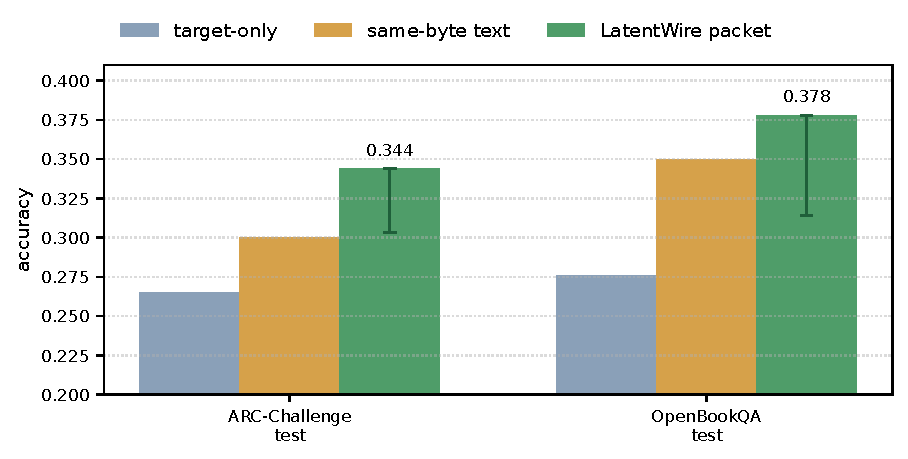
\includegraphics[width=0.92\linewidth]{figures/accuracy_overview.pdf}
  \caption{Packet accuracy against target-only and same-byte structured text controls. Error bars show the lower paired-bootstrap lift above target-only; upper uncertainty is omitted for readability because the gate is one-sided.}
  \label{fig:accuracy}
\end{figure}

On \arc{}, the matched Fourier/anchor-syndrome packet reaches 0.344 mean test accuracy with minimum seed accuracy 0.342. The answer-key-forbidden source choice itself reaches 0.346, and packet predictions match the source-selected candidate at 0.995 mean rate across seeds. Anchor-ID shuffle, anchor-value shuffle, and spectral-bin permutation controls all fail in 0/10 seeds and collapse near target-only. The random shared-anchor diagnostic passes, which weakens any claim that named anchors are semantically special, but strengthens the claim that a shared public coordinate chart is the relevant mechanism.

On \obqa{}, the 3-byte packet reaches 0.378--0.380 across seeds, matching the source-choice accuracy of 0.378. The largest candidate-derangement control accuracy is 0.212, and the minimum lift over same-byte structured text is +0.028. This second task matters because it reduces the risk that the result is only an \arc{} artifact, though it is still a same-family packet result rather than a cross-family result.

\section{Falsification and failure decomposition}

The most important negative result is the Phi-3 source-family replacement. We keep the same \arc{} packet budget, public basis, seed count, and bootstrap budget, but replace the Qwen source-choice cache with a Phi-3 source. The packet no longer passes. On the full \arc{} test slice, the Phi-3 packet reaches 0.244 versus target-only 0.265. On the stricter Qwen-disagreement slice, where the alternate source and Qwen source disagree, the Phi-3 packet reaches 0.200 versus 0.340 for the Qwen-substituted packet.

\begin{table}[t]
  \centering
  \small
  \setlength{\tabcolsep}{3.4pt}
  \begin{tabular}{llrrrrrl}
    \toprule
    Source & surface & n & packet & target & text & ref. pkt & blocker \\
    \midrule
    Phi-3 & full test & 1172 & 0.244 & 0.265 & 0.232 & -- & source quality \\
    Phi-3 & Qwen-disagree & 833 & 0.200 & 0.273 & 0.203 & 0.340 & source quality \\
    TinyLlama & Qwen-disagree & 473 & 0.269 & 0.268 & 0.258 & 0.317 & family mismatch \\
    Qwen2.5-1.5B & full test & 1172 & 0.442 & 0.265 & 0.401 & -- & val incomplete \\
    \bottomrule
  \end{tabular}
  \caption{Cross-family and source-family diagnostics. ``Ref. pkt'' is the Qwen-substituted packet on disagreement rows. Qwen2.5-1.5B is encouraging but same-family and validation-incomplete, so it is not a headline cross-family claim.}
  \label{tab:falsification}
\end{table}

The failure decomposition separates three causes: source endpoint quality, packet corruption, and common-feature mismatch. For Phi-3, packet predictions follow the Phi-3 source choice at 0.997, but the source itself is below the target. For TinyLlama, packet fidelity is also high, but the source-family mismatch causes the disagreement-slice packet to lose to Qwen-substituted packets. For Qwen2.5-1.5B, the source is stronger and the packet is useful on frozen test, but the validation disagreement gate is incomplete. Across these rows, the packet mostly transports the source-selected candidate through the public coordinate basis. The next research gate is therefore not another scalar packet shuffle; it is either an explicit comparison to source-index/score packets or a richer common-feature connector that can beat packet-only source choice.

We also tested cached learned repairs on the available local artifacts. A candidate-syndrome connector that sees packet and score-shape features reaches 0.288 versus 0.317 for Qwen-substituted packets on frozen TinyLlama/Qwen disagreement rows. A one-hidden-layer MLP over cached TinyLlama hidden/query summaries reaches 0.232, below Qwen-substituted packets, cached Tiny packets, target-only, and same-byte text. These negatives are useful: simple cached score geometry and mean hidden/query summaries do not explain the remaining oracle headroom.

\section{Systems boundary}

The systems contribution is byte/exposure accounting, not native serving throughput. Figure~\ref{fig:systems} compares framed packet bytes with one-token KV/cache-state accounting floors from neighboring systems and quantization methods. \method{} sends 6--11 framed bytes on the two headline rows. A one-token 1-bit-per-KV-element accounting floor is 768 bytes in our model-configuration accounting; the largest headline packet is therefore 69.8x smaller than that floor. C2C-style cache transfer, KVComm-style selective sharing, and serving substrates such as vLLM/PagedAttention and SGLang operate on KV/cache objects rather than task-level packets~\citep{Fu2025C2C,Shi2025KVComm,Kwon2023vLLM,Zheng2023SGLang}. KV quantization work reduces cache bytes but still communicates or stores model state~\citep{Zandieh2024QJL,Liu2024KIVI,Hooper2024KVQuant,Zandieh2025TurboQuant}.

\begin{figure}[t]
  \centering
  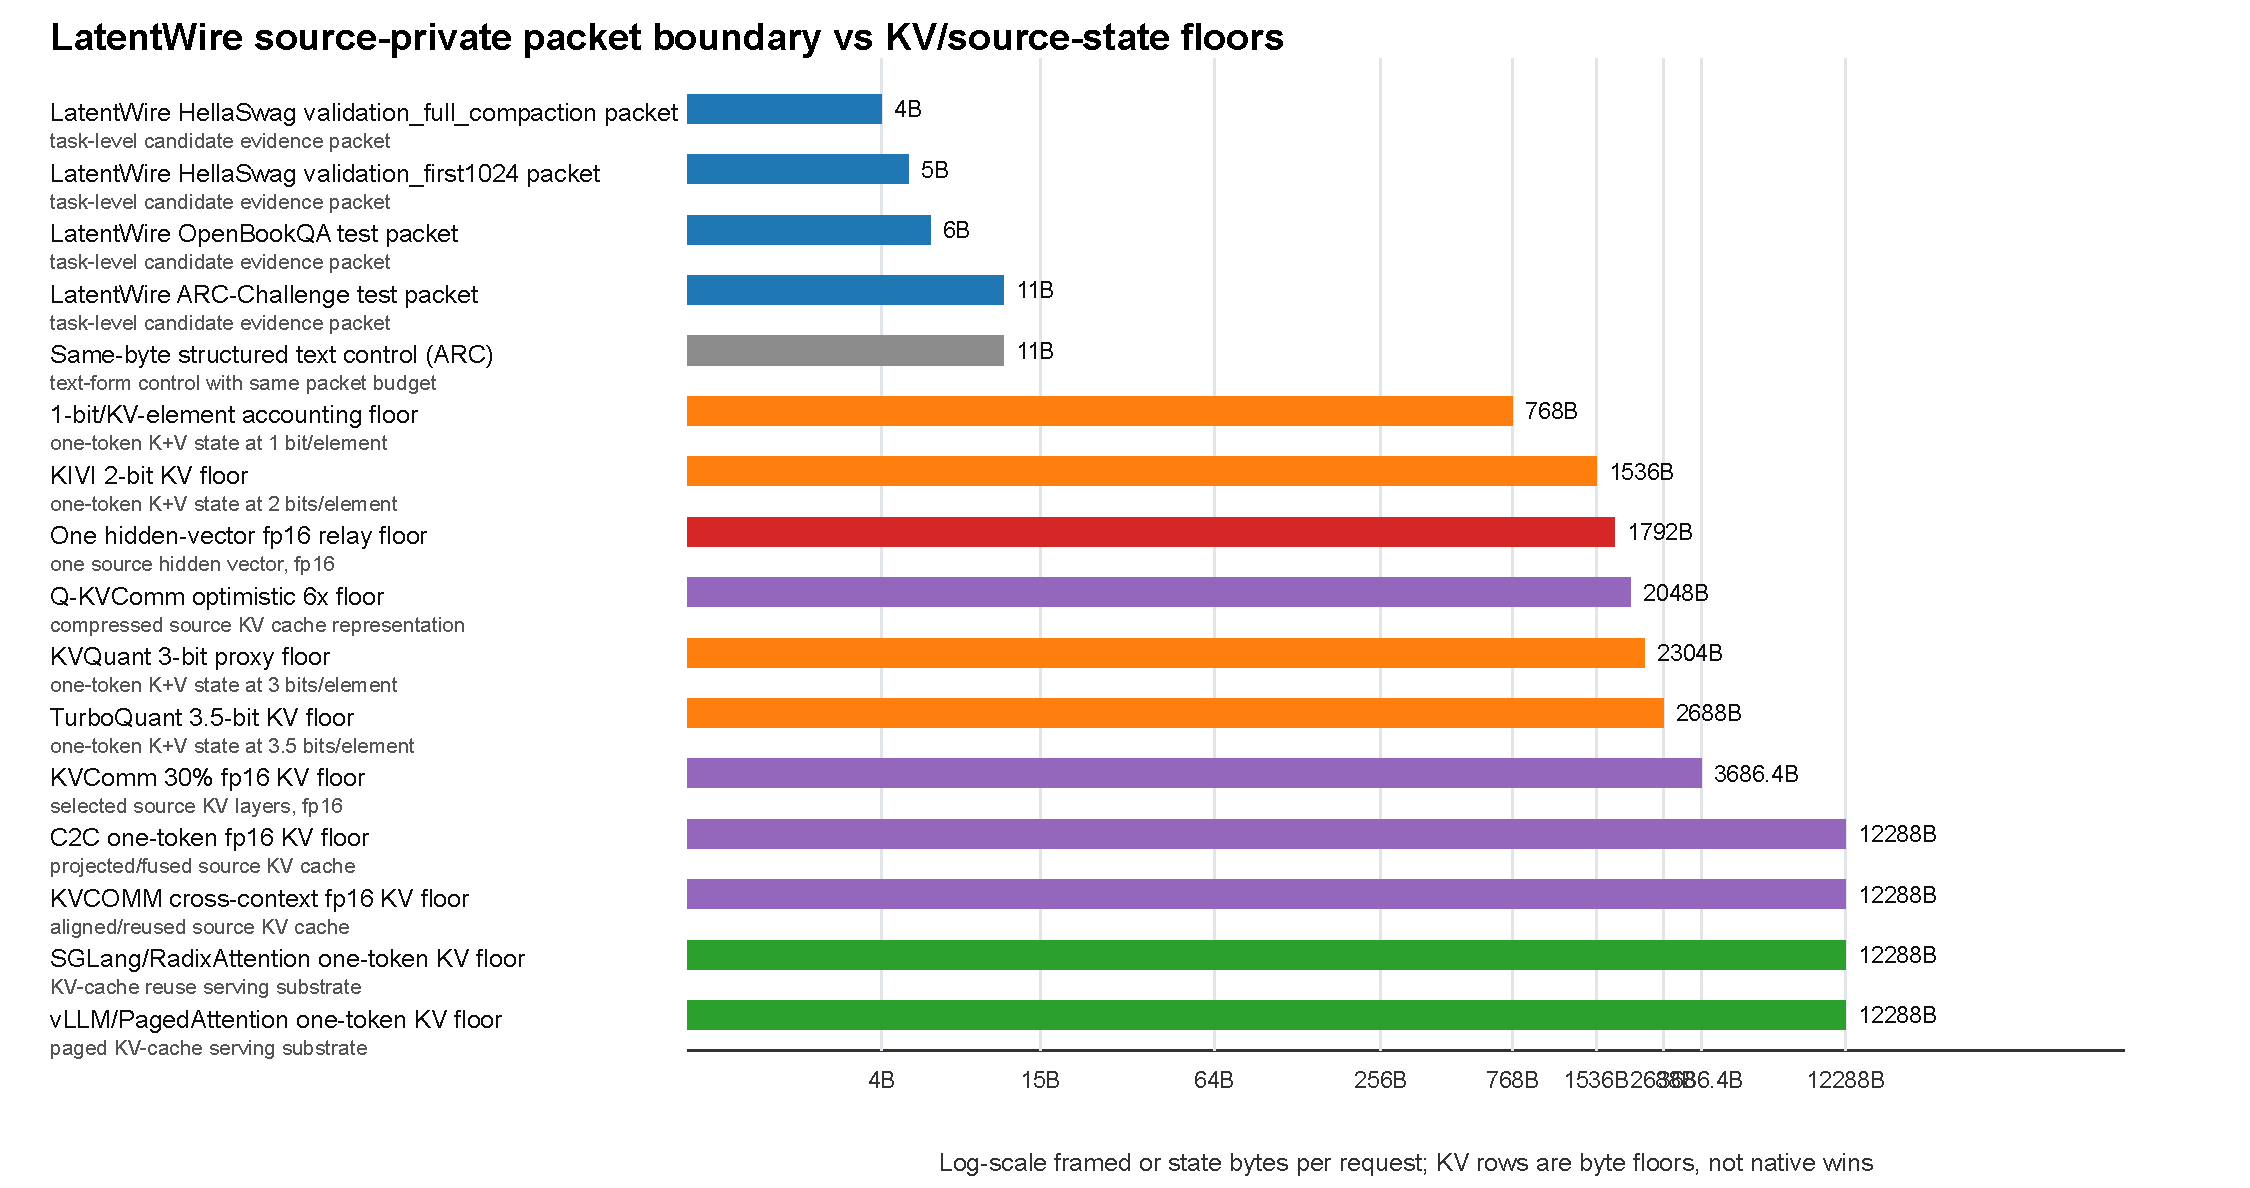
\includegraphics[width=0.95\linewidth]{figures/systems_boundary.pdf}
  \caption{Boundary-byte accounting. Packet rows are measured task-packet objects. KV/cache rows are lower-bound floors or neighboring serving substrates, not native speed comparisons.}
  \label{fig:systems}
\end{figure}

\begin{table}[t]
  \centering
  \small
  \setlength{\tabcolsep}{3.8pt}
  \begin{tabular}{lrrlll}
    \toprule
    Method & raw & framed & text & KV/hidden & claim status \\
    \midrule
    \method{} \obqa{} packet & 3B & 6B & no & no & local positive \\
    \method{} \arc{} packet & 8B & 11B & no & no & local positive \\
    Same-byte text control & 8B & 11B & yes & no & control only \\
    1-bit/KV-element floor & 768B & 768B & no & KV & floor only \\
    KIVI 2-bit KV floor & 1536B & 1536B & no & KV & floor only \\
    C2C one-token KV floor & 12288B & 12288B & no & KV & native pending \\
    \bottomrule
  \end{tabular}
  \caption{Exposure classes. The paper-ready systems claim is that the communicated object is much smaller and less exposing than KV/cache-state objects under this accounting. It is not a GPU throughput, TTFT, TPOT, or HBM claim.}
  \label{tab:systems}
\end{table}

\section{Related work}

\textbf{Latent and relative representation communication.} Relative representations use similarities to anchors to enable latent-space communication under invariances~\citep{Moschella2023Relative}. Sparse autoencoders and feature-space universality work motivate common-feature interfaces~\citep{Cunningham2023SAE,Engels2024SAEUniversality}. SAEBench provides evaluation machinery for sparse autoencoders~\citep{Karvonen2025SAEBench}, but these works do not by themselves provide a packet protocol or task-level evidence transfer result.

\textbf{Prompt compression and learned prefixes.} Prefix tuning and gist tokens learn continuous or discrete prompt-like interfaces within language models~\citep{Li2021Prefix,Mu2023Gist}. \method{} differs because the communicated object is a byte packet decoded by a public receiver, not a learned soft prompt injected into one target. Query-bottleneck connectors such as BLIP-2's Q-Former show that learned bottlenecks can bridge frozen model families across modalities~\citep{Li2023BLIP2}; our failed cached hidden/query summaries suggest that a true tokenwise query-bottleneck is the right future branch, but it is not closed here.

\textbf{Cache communication and systems.} Cache-to-cache and selective KV-sharing systems communicate richer internal state and are the closest competitors for model-to-model communication~\citep{Fu2025C2C,Shi2025KVComm}. vLLM and SGLang improve serving through KV-cache management and reuse~\citep{Kwon2023vLLM,Zheng2023SGLang}. KV quantizers such as QJL, KIVI, KVQuant, and TurboQuant reduce state cost but remain state-transfer or state-storage techniques~\citep{Zandieh2024QJL,Liu2024KIVI,Hooper2024KVQuant,Zandieh2025TurboQuant}. Our current systems result is a boundary artifact against these state objects, not a native throughput win.

\section{Limitations and next gate}

The main limitation is scope. The positive results are same-family/source-cache results on public multiple-choice tasks, and the packet largely preserves the source's selected candidate. We therefore do not claim to beat explicit source-index communication, source-score quantization, or calibrated source-choice baselines; those are required before a stronger compression claim. Phi-3 cross-family replacement fails, TinyLlama common-feature repair fails, and a true cross-family learned query-bottleneck remains future work. We also do not claim superiority over C2C, KVComm, QJL, KIVI, TurboQuant, vLLM, or SGLang in native serving metrics. Those rows require NVIDIA hardware and matched implementations.

The next exact gate for an ICLR-strength claim is a frozen-endpoint tokenwise connector with an explicit byte or query budget, tested against C2C/KV-style and structured-text baselines, with source-destroying controls and strict same-family versus cross-family separation. The current strongest claim is narrower: fixed-byte source-private packets can transfer useful same-family evidence on \arc{} and \obqa{}, and the accompanying falsification ladder clarifies where the method stops working.

\section{Conclusion}

\method{} shows that a tiny source-private candidate packet can improve frozen receiver decisions on two public QA benchmarks under strict same-family controls. The same evidence also draws a hard boundary: the current method is mostly source-choice preserving, is not a universal latent language, and does not yet solve cross-family communication. This combination of positive packet transfer, negative falsification, and systems byte/exposure accounting is the paper's core.

\bibliography{latentwire_colm2026}
\bibliographystyle{colm2026_conference}

\appendix

\section{Artifact manifest}

\begin{itemize}
\item \arc{} headline: \url{results/source_private_arc_challenge_fourier_anchor_syndrome_gate_20260502_budget8_10seed_b2000}.
\item Phi-3 falsification: \url{results/source_private_arc_challenge_source_family_cache_falsification_20260502_phi3_cpu_budget8_10seed_b2000}.
\item Cross-family decomposition: \url{results/source_private_arc_cross_family_failure_decomposition_20260502}.
\item Systems boundary: \url{results/source_private_systems_boundary_figure_table_20260502}.
\item \obqa{} headline: \url{results/source_private_openbookqa_seed_stability_20260501_qwen05_hashed_test_3b}.
\end{itemize}

\section{Reproducibility summary}

The artifact bundle records exact shell commands, input hashes, output hashes,
and rerun results. The paper rows are produced from cached,
answer-key-forbidden source-choice artifacts with the following settings:

\begin{center}
\scriptsize
\begin{tabular}{llll}
\toprule
Row & script & seeds & key settings \\
\midrule
\arc{} & Fourier/anchor syndrome gate & 10 & 8B, 2000 bootstraps \\
\obqa{} & seed-stability gate & 5 & 3B, hashed features, 500 bootstraps \\
Phi-3 & source-family cache falsification & 10 & 8B, cached Phi-3 source \\
Systems & systems boundary table & -- & byte/exposure accounting only \\
\bottomrule
\end{tabular}
\end{center}

The reruns are metric-reproducible, but not intended to be byte-identical:
JSON files contain creation times and several artifacts include measured local
latencies.

\section{Lay explanation of the main experiment}

The experiment asks whether one model can send a tiny hint to another model. Both models see the same question and answer choices. The sender chooses a compressed coordinate hint, only a few bytes long. The receiver uses that hint to choose an answer. If both sides agree on the coordinate system, the hint helps. If we scramble the coordinate system, the hint stops helping. That is evidence for a real shared packet interface on the tested same-family setting, while the failed Phi-3 run shows the interface is not yet general across model families.

\end{document}
